\documentclass[11pt]{article}

\usepackage[utf8]{inputenc} % character encoding - you don't need to understand this

% Note that if you want to make a number sign, you need to type \#
% below are a bunch of useful packages, it doesn't cost anything to include them all so you might as well
\usepackage{amsmath}		            % lets you input equations in math mode
\usepackage{graphicx}		            % lets you include images
\usepackage{enumerate}		            % lets you make lists
\usepackage{subcaption}                 % if you want to use subcaptions
\usepackage[colorlinks=true]{hyperref}  % for making hyperlinks
\usepackage{hypcap}	                    % makes links refer to figures and not captions
\usepackage{relsize}		            % lets you use relative font sizes
\usepackage{caption}                    % lets you add captions
\usepackage{array}                      % lets you specify table column widths
\usepackage[margin=1in, paperwidth=8.5in, paperheight=11in]{geometry}
\usepackage{listings}
\usepackage{float}
\usepackage{tabularx}
\usepackage{textgreek}
\usepackage{amssymb}
\usepackage{amsthm}
\usepackage{placeins}
\usepackage{imakeidx}
\renewcommand{\qedsymbol}{$\blacksquare$}
\usepackage{blindtext}
\usepackage{csquotes}
\usepackage[style=numeric-comp,sorting=none]{biblatex}
% \usepackage{biblatex}
\addbibresource{thesis.bib}
\makeindex[columns=2, title=Alphabetical Index, 
options= -s example_style.ist, intoc]

% Note that if you want to make a number sign, you need to type \#
\hypersetup{
    colorlinks=true,
    linkcolor=blue,
    filecolor=magenta,
    urlcolor=cyan,
}

\lstdefinestyle{mystyle}{
  backgroundcolor=\color{backcolour},   commentstyle=\color{codegreen},
  keywordstyle=\color{magenta},
  numberstyle=\tiny\color{codegray},
  stringstyle=\color{codepurple},
  basicstyle=\ttfamily\footnotesize,
  breakatwhitespace=false,         
  breaklines=true,                 
  captionpos=b,                    
  keepspaces=true,                 
  numbers=left,                    
  numbersep=5pt,                  
  showspaces=false,                
  showstringspaces=false,
  showtabs=false,                  
  tabsize=2
}

\begin{document}
\title{Mixed Analog-Digital VLSI Mini-Project I: 2-Input AND Gate}
\author{Qingmu Deng}
\maketitle % this line makes the title appear, along with today's date, automatically updated.

\section*{Project Links}

Project Github: \href{https://github.com/QingmuDeng/MADVLSI/tree/main/mini1}{https://github.com/QingmuDeng/MADVLSI/tree/main/mini1}

\noindent
Project zip file: \href{https://github.com/QingmuDeng/MADVLSI/blob/main/mini1/Deng-mini1.zip?raw=true}{https://github.com/QingmuDeng/MADVLSI/blob/main/mini1/Deng-mini1.zip?raw=true}
\section{Schematic Capture and Simulation}
    \begin{figure}[!ht]
        \begin{subfigure}{0.5\linewidth}
            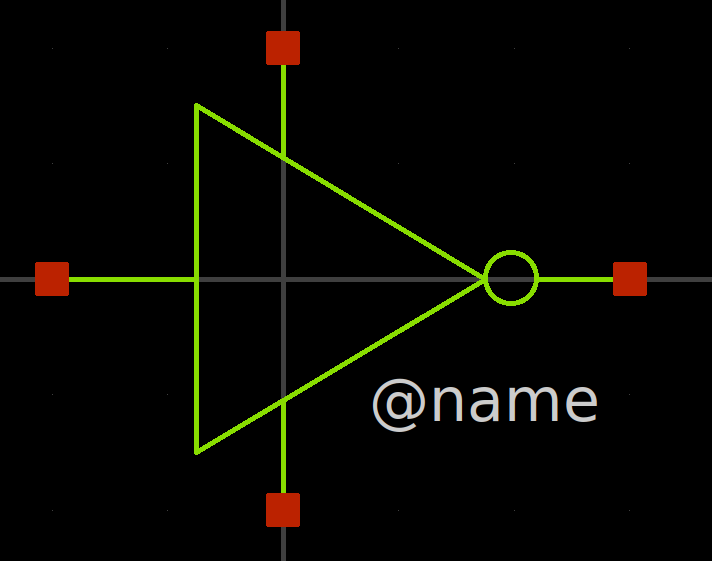
\includegraphics[width=\linewidth]{../img/inverter_sym.png}
            \caption{Inverter symbol created in Xschem.}
        \end{subfigure}
        \begin{subfigure}{0.5\linewidth}
            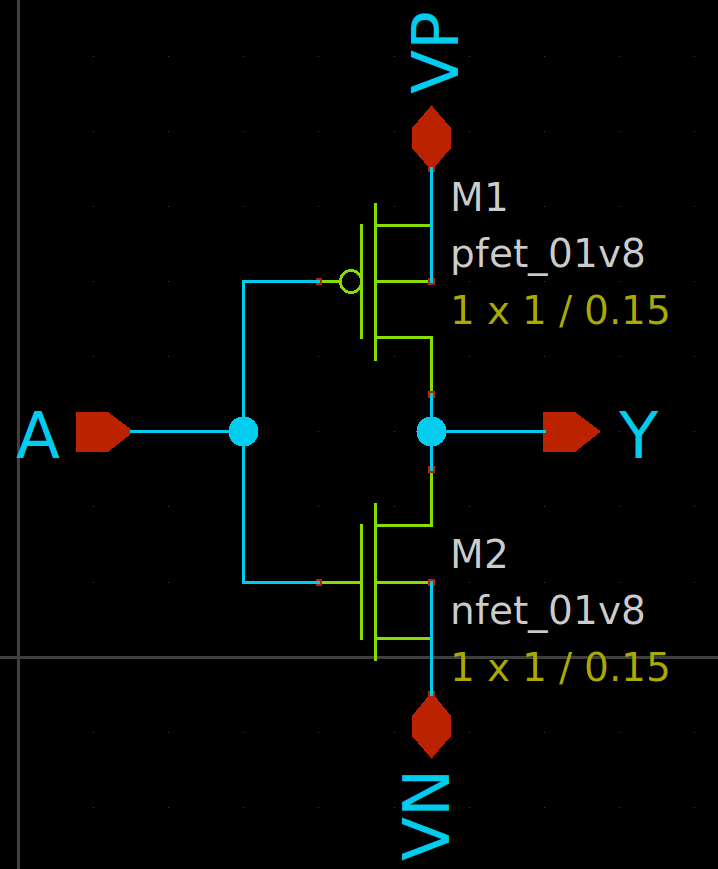
\includegraphics[width=\linewidth]{../img/inverter_sch.png}
            \caption{Inverter schematic created in Xschem.}
        \end{subfigure}
        \caption{Inverter design in Xschem.}
        \label{fig:inv}
    \end{figure}
    To begin with, I implemented an inverter design shown in Figure \ref{fig:inv} as introduced by Professor Minch in his tutorial video.
    \begin{figure}[!ht]
        \begin{subfigure}{0.5\linewidth}
            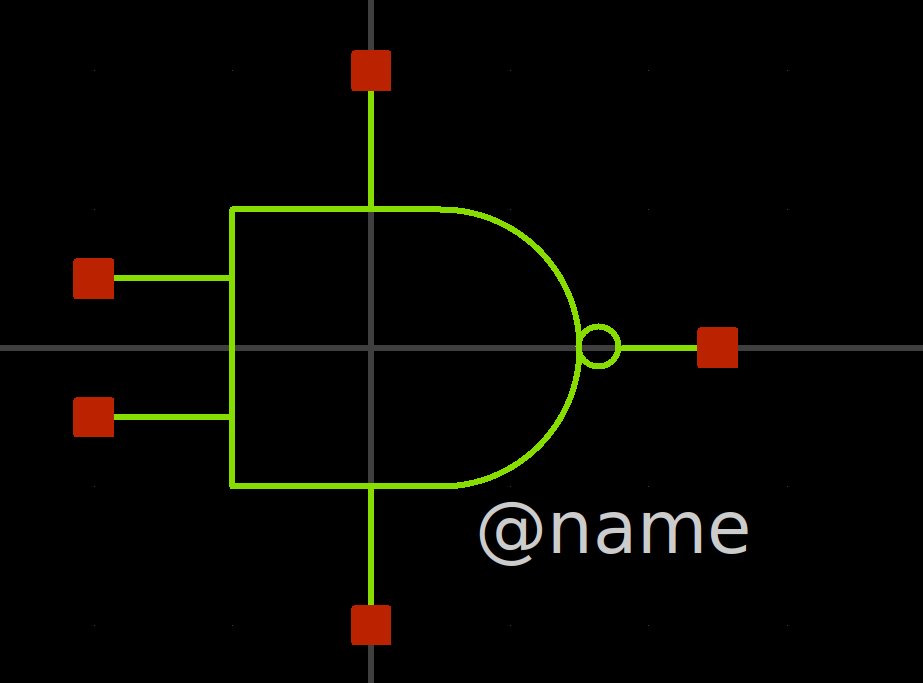
\includegraphics[width=\linewidth]{../img/NAND2_sym.png}
            \caption{NAND2 symbol created in Xschem.}
        \end{subfigure}
        \begin{subfigure}{0.5\linewidth}
            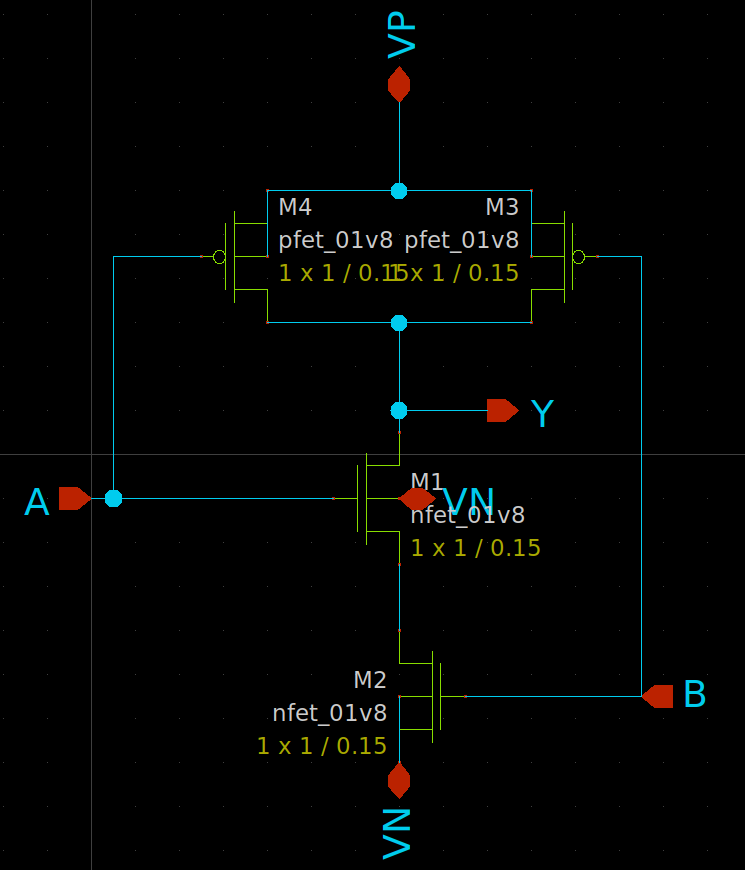
\includegraphics[width=\linewidth]{../img/NAND2_sch.png}
            \caption{NAND2 schematic created in Xschem.}
        \end{subfigure}
        \caption{NAND2 design in Xschem.}
        \label{fig:nand2}
    \end{figure}
    Similarly, I independently created a hierarchy schematic for NAND2 as shown in Figure \ref{fig:nand2}.

    \FloatBarrier
    I created an AND2 gate by inverting the output of NAND2 with the inverter. You can see the test harness of the AND2 gate in Figure \ref{fig:and2}. $V_{DD}$ is set to be 1.8 $V$, and the square waves at NAND2 inputs switches between 0 $V$ and 1.8 $V$. To capture all four possible inputs, $\{00,\ 01,\ 10,\ 11\}$, to be presented to this two-input gate, the square wave at the input node $V_B$ is set to have twice the period of $V_A$. The output node $V_{out}$ is loaded with a 200 $fF$ capacitor as specified.
    \begin{figure}[!ht]
        % \begin{subfigure}{0.5/textwidth}
        %     \
        % \end{subfigure}
        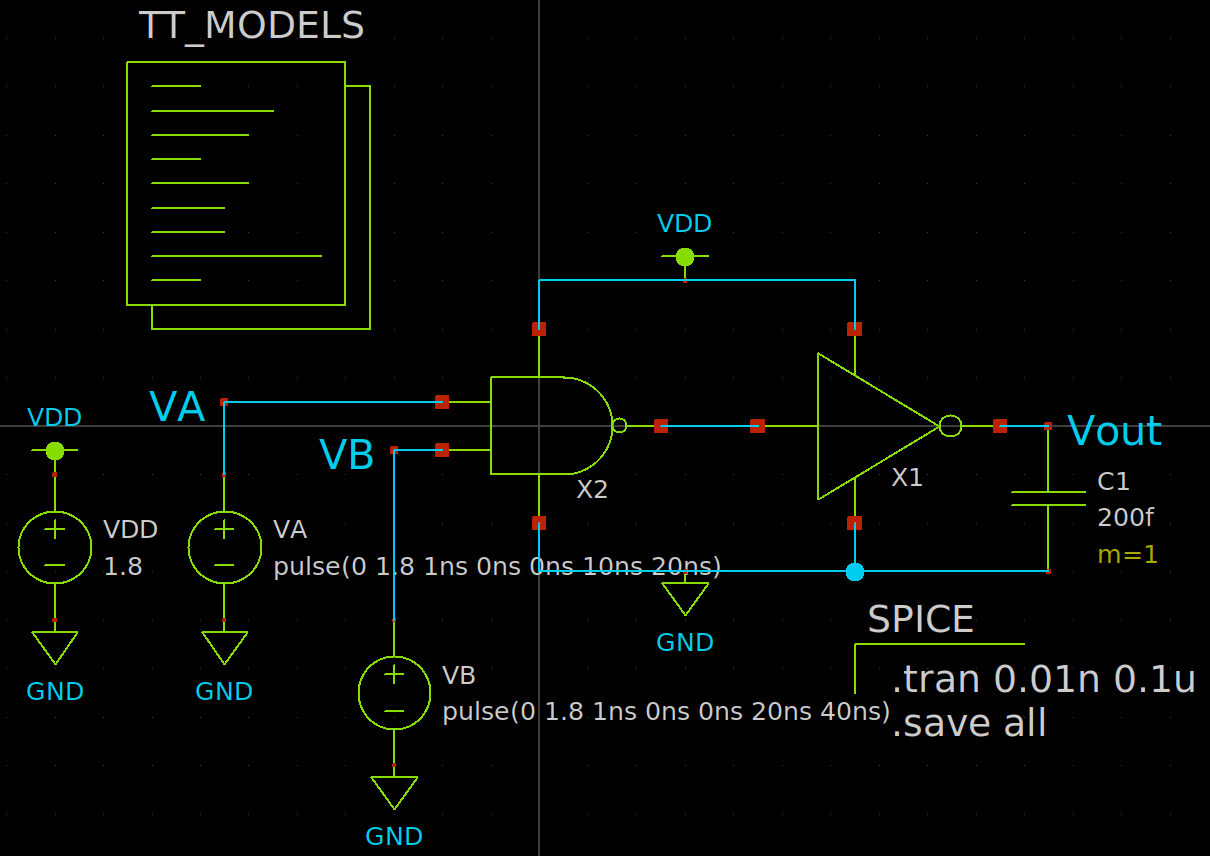
\includegraphics[width=\linewidth]{../img/AND2_harness.png}
        \caption{The simulation setup of a AND2 gate made of a NAND2 and an inverter.}
        \label{fig:and2}
    \end{figure}

    As you can see for the simulation results in Figure \ref{fig:and2res}, the only time where $V_{out}$ outputs high is when both $V_A$ and $V_B$ outputs high. This follows out expectation of how an AND2 gate should behave.
	\begin{figure}[!ht]
        % \begin{subfigure}{0.5/textwidth}
        %     \
        % \end{subfigure}
        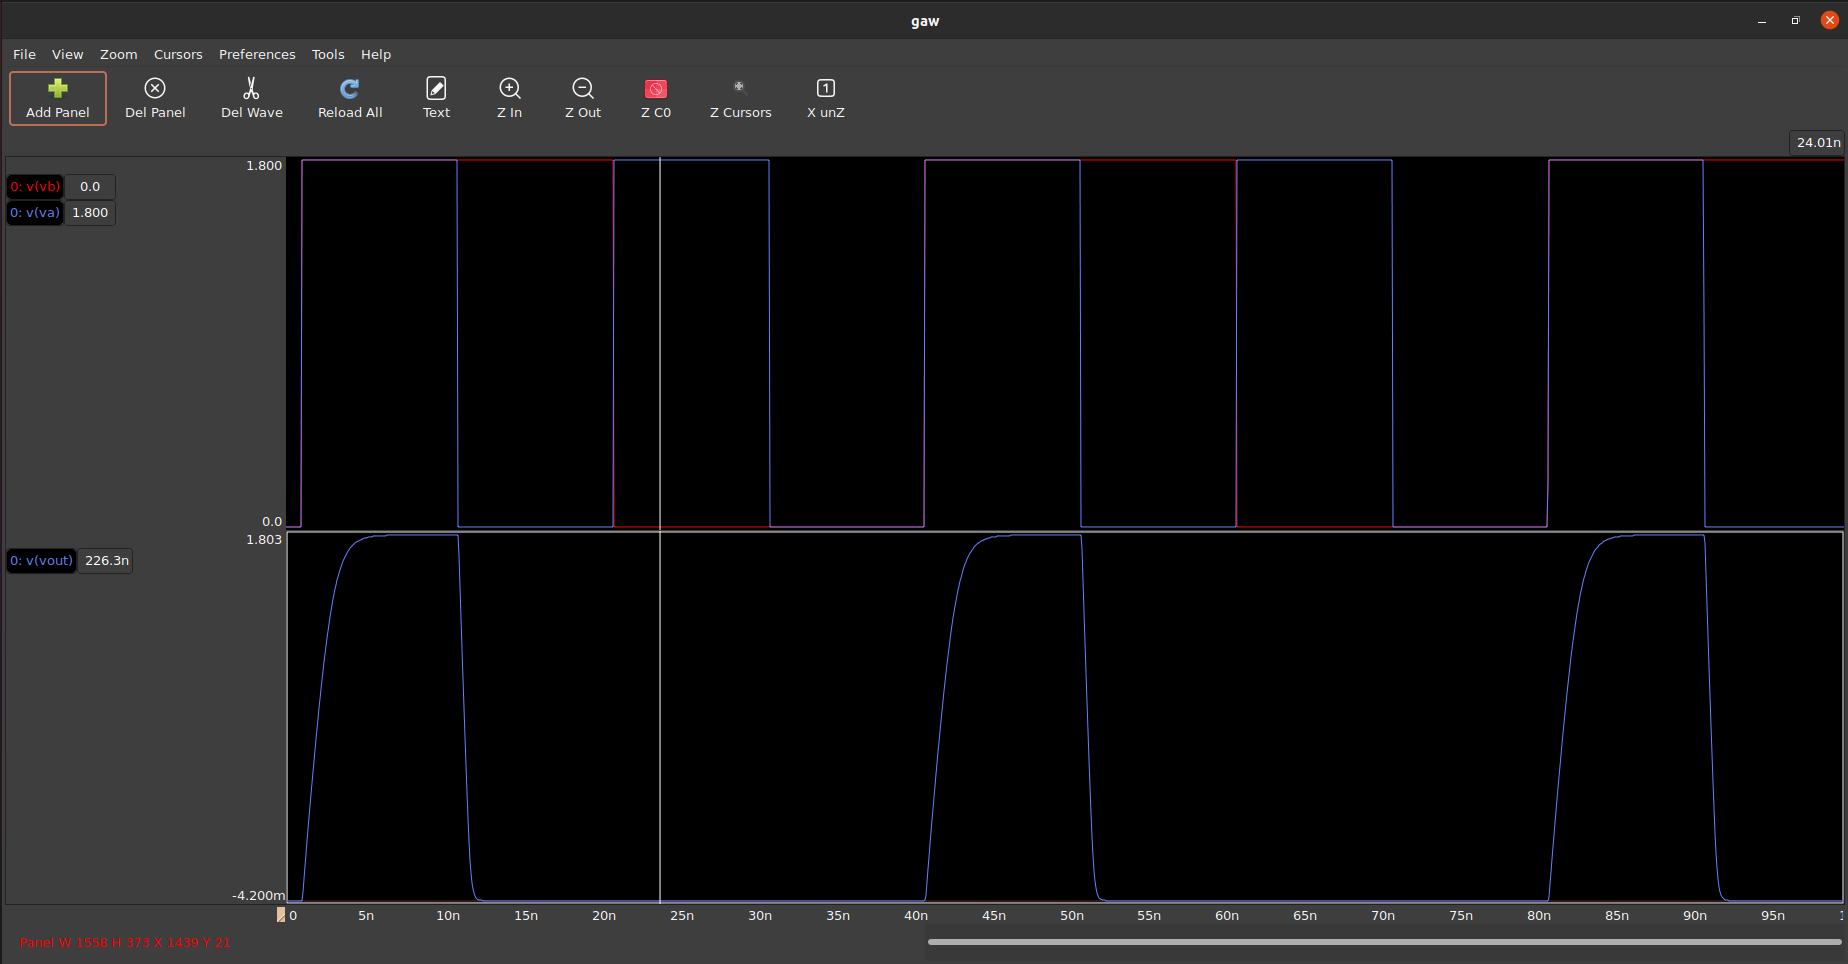
\includegraphics[width=\linewidth]{../img/AND2_sim.png}
        \caption{The simulation AND2 gate behavior viewed in \textit{gaw}.}
        \label{fig:and2res}
    \end{figure}


\FloatBarrier
\section{Layout Design}
    Similarly, the inverter and NAND2 were separately laid out in \textit{Magic} as shown in Figure \ref{fig:invmag} and \ref{fig:nand2mag}. The output of the NAND2 was designed to align with the input of the inverter such that they can fit together nicely to form AND2 as shown in Figure \ref{fig:and2mag}, all the while sharing and extending the same power rails.
    \begin{figure}[!ht]
        \centering
        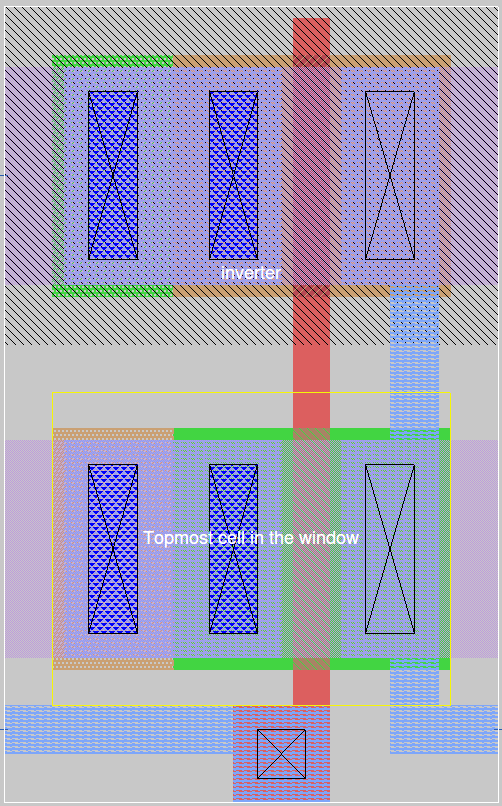
\includegraphics[width=0.8\linewidth]{../img/inverter_mag.png}
        \caption{\textit{Magic} layout of the inverter.}
        \label{fig:invmag}
    \end{figure}
    \begin{figure}[!ht]
        \centering
        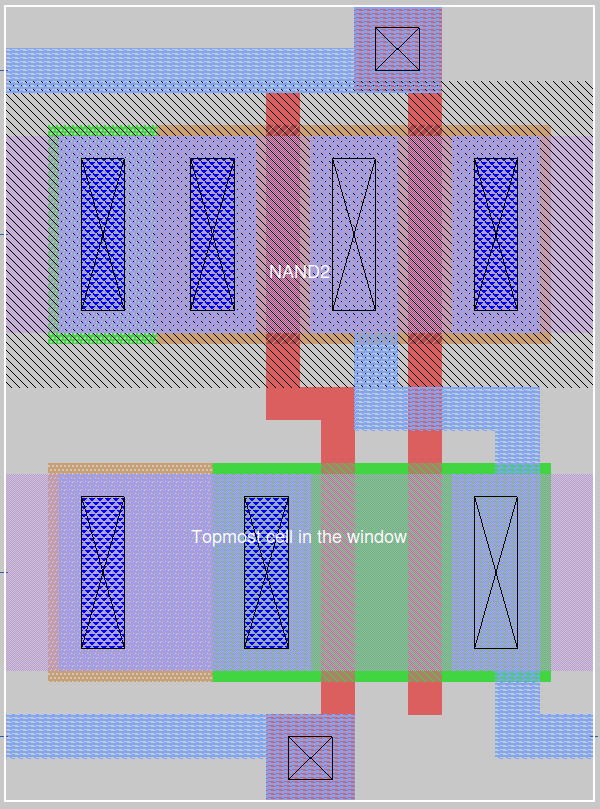
\includegraphics[width=0.8\linewidth]{../img/nand2_mag.png}
        \caption{\textit{Magic} layout of the NAND2.}
        \label{fig:nand2mag}
    \end{figure}
    \begin{figure}[!ht]
        \centering
        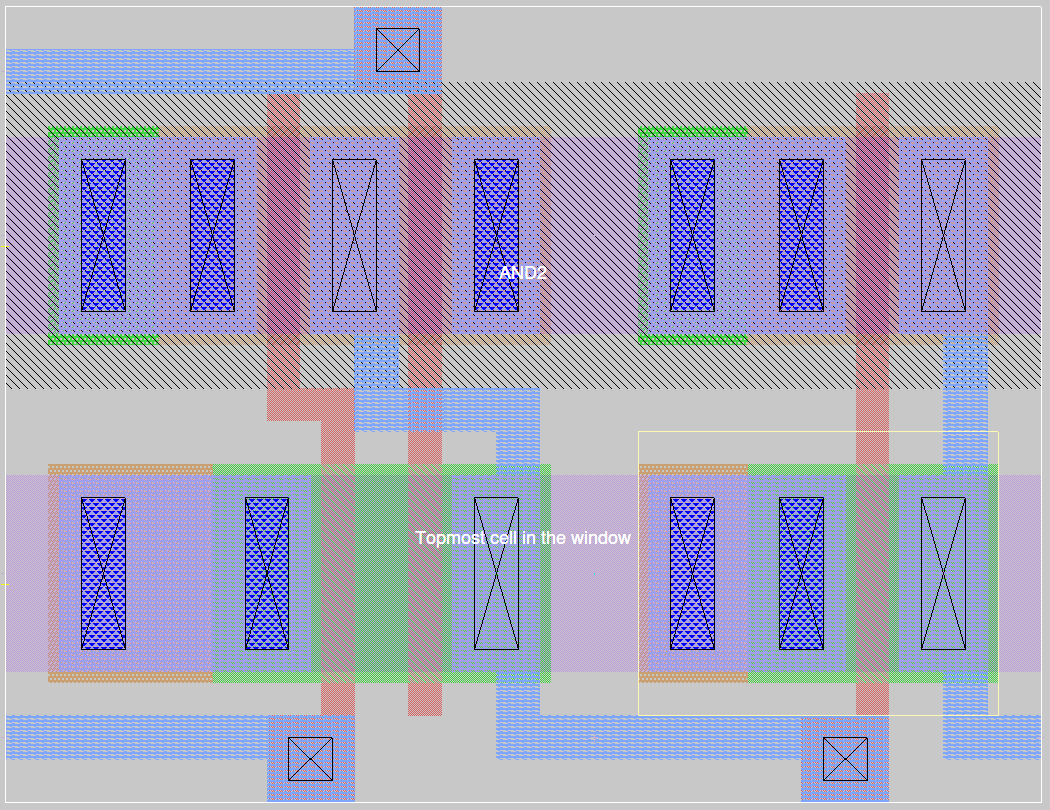
\includegraphics[width=\linewidth]{../img/and2mag.png}
        \caption{\textit{Magic} layout of the AND2 by combining NAND2 and inverter layouts.}
        \label{fig:and2mag}
    \end{figure}

    \FloatBarrier
    \section{Layout versus Schematic}
    Finally, I compared the two netlists generated through schematic capture and physical layout. The output of the LVS can be found below. The netlists of the two designs were found to be uniquely matching. Although there are two mismatches highlighted, they are spurious as they are simply a permutation of the input pins. As suggested by the LVS output at the end of the block where the two mismatches were reported, the two NAND gate netlists were equivalent.
    \begin{lstlisting}[language=tcl, caption=Netgen comparison between Xschem and Magic AND2]
Equate elements:  no current cell.
Equate elements:  no current cell.

Subcircuit summary:
Circuit 1: inverter                        |Circuit 2: inverter                        
-------------------------------------------|----------------------------
sky130_fd_pr__pfet_01v8 (1)                |sky130_fd_pr__pfet_01v8 (1)                
sky130_fd_pr__nfet_01v8 (1)                |sky130_fd_pr__nfet_01v8 (1)                
Number of devices: 2                       |Number of devices: 2                       
Number of nets: 4                          |Number of nets: 4                          
------------------------------------------------------------------------
Circuits match uniquely.
Netlists match uniquely.

Subcircuit pins:
Circuit 1: inverter                        |Circuit 2: inverter                        
-------------------------------------------|----------------------------
Y                                          |Y                                          
A                                          |A                                          
VN                                         |VN                                         
VP                                         |VP                                         
------------------------------------------------------------------------
Cell pin lists are equivalent.
Device classes inverter and inverter are equivalent.

Subcircuit summary:
Circuit 1: NAND2                           |Circuit 2: NAND2                           
-------------------------------------------|----------------------------
sky130_fd_pr__nfet_01v8 (2)                |sky130_fd_pr__nfet_01v8 (2)                
sky130_fd_pr__pfet_01v8 (2)                |sky130_fd_pr__pfet_01v8 (2)                
Number of devices: 4                       |Number of devices: 4                       
Number of nets: 6                          |Number of nets: 6                          
------------------------------------------------------------------------
Circuits match uniquely.
Netlists match uniquely.

Subcircuit pins:
Circuit 1: NAND2                           |Circuit 2: NAND2                           
-------------------------------------------|----------------------------
VP                                         |VP                                         
B                                          |A **Mismatch**                             
A                                          |B **Mismatch**                             
VN                                         |VN                                         
Y                                          |Y                                          
------------------------------------------------------------------------
Cell pin lists are equivalent.
Device classes NAND2 and NAND2 are equivalent.

Subcircuit summary:
Circuit 1: AND_no_C.spice                  |Circuit 2: layout/AND2.spice               
-------------------------------------------|----------------------------
inverter (1)                               |inverter (1)                               
NAND2 (1)                                  |NAND2 (1)                                  
Number of devices: 2                       |Number of devices: 2                       
Number of nets: 6                          |Number of nets: 6                          
------------------------------------------------------------------------
Circuits match uniquely.
Netlists match uniquely.
Cells have no pins;  pin matching not needed.
Device classes AND_no_C.spice and layout/AND2.spice are equivalent.
Circuits match uniquely.

    \end{lstlisting}
    
\end{document}
